\documentclass[a4paper]{article}

\usepackage[portuguese]{babel}
\usepackage[utf8]{inputenc}
\usepackage[T1]{fontenc}

\newcommand{\documentTitle}{Braitenberg Vehivles} %Macro definition
\newcommand{\documentAuthors}{João Rafael (2008111876) \and José Ribeiro (2008112181)} %Macro definition

\title{\documentTitle}
\author{\documentAuthors{}}

\usepackage{hyperref}
\hypersetup{
	pdftitle = \documentTitle
	,pdfauthor = \documentAuthors
	,pdfsubject = {Introduction to Artificial Inteligence Project \#1 Report}
	,pdfkeywords = {Artificial Inteligence Project} {Reactive Agents} {Braitenberg Vehicles}
	,pdfborder = {0 0 0}
}

\usepackage{wrapfig}
\usepackage{array}
\usepackage{anysize}
\usepackage{lscape}
\usepackage[pdftex]{graphicx}

\marginsize{3.5cm}{3.5cm}{3cm}{3cm}

\makeatletter

\begin{document}
\maketitle
\cleardoublepage

\tableofcontents
\cleardoublepage


\setlength{\parindent}{1cm}
\setlength{\parskip}{0.3cm}

\section{Introduction}
% TODO

\cleardoublepage
\section{Breve Libraries}
% TODO
OBB Sphere distance

Activators

Constructors with parameters

Sensor rotation/initialization

Multibody collision handlers (Proxies, and Real's parents )

\cleardoublepage
\section{Sensors}

\subsection{Light}

\begin{wrapfigure}{r}{0.5\textwidth}
	\vspace{-30pt}
	\begin{center}
		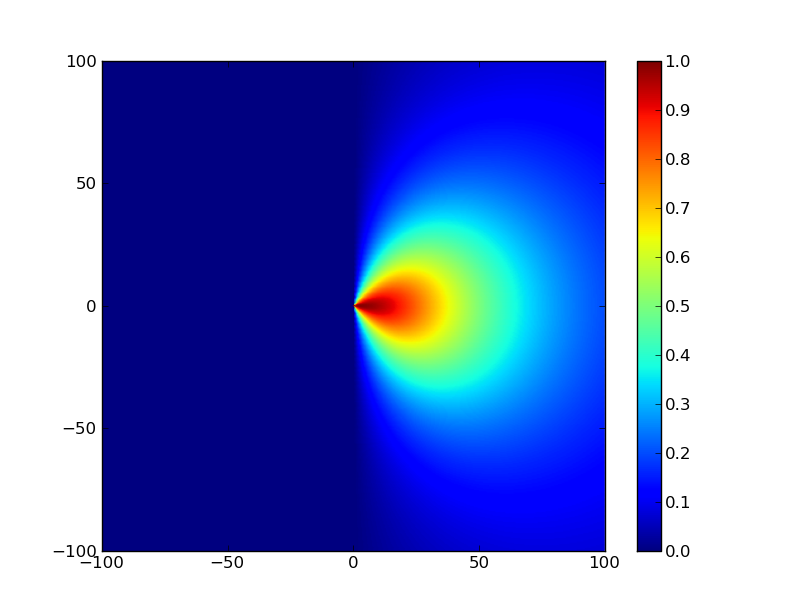
\includegraphics[width=0.48\textwidth]{graphs/light.png}
	\end{center}
	\vspace{-30pt}
	\caption{Light: $bias=50$ $\alpha=\pi/2$}
\end{wrapfigure}

\subsection{Distance}
\begin{wrapfigure}{r}{0.5\textwidth}
	\vspace{-30pt}
	\begin{center}
		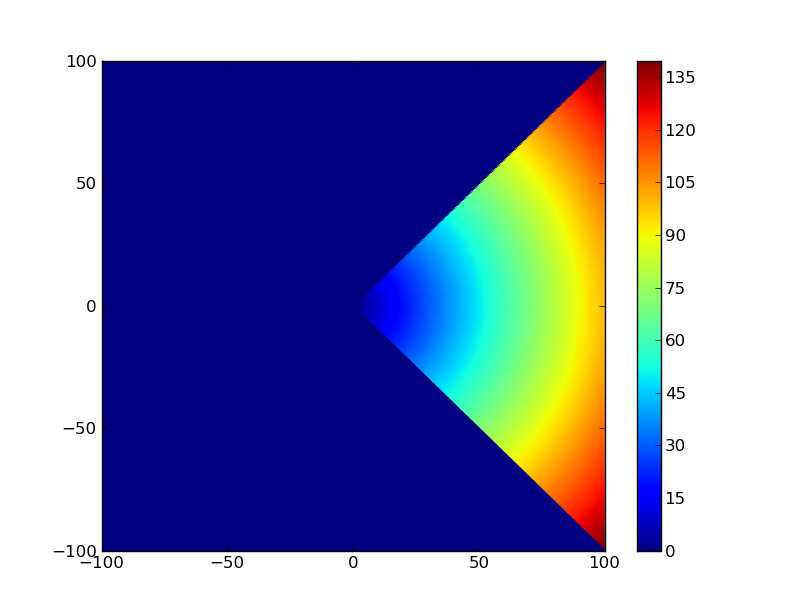
\includegraphics[width=0.48\textwidth]{graphs/distance.png}
	\end{center}
	\vspace{-30pt}
	\caption{Distance: $\alpha=\pi/4$}
\end{wrapfigure}

\subsection{Proximity}
\begin{wrapfigure}{r}{0.5\textwidth}
	\vspace{-30pt}
	\begin{center}
		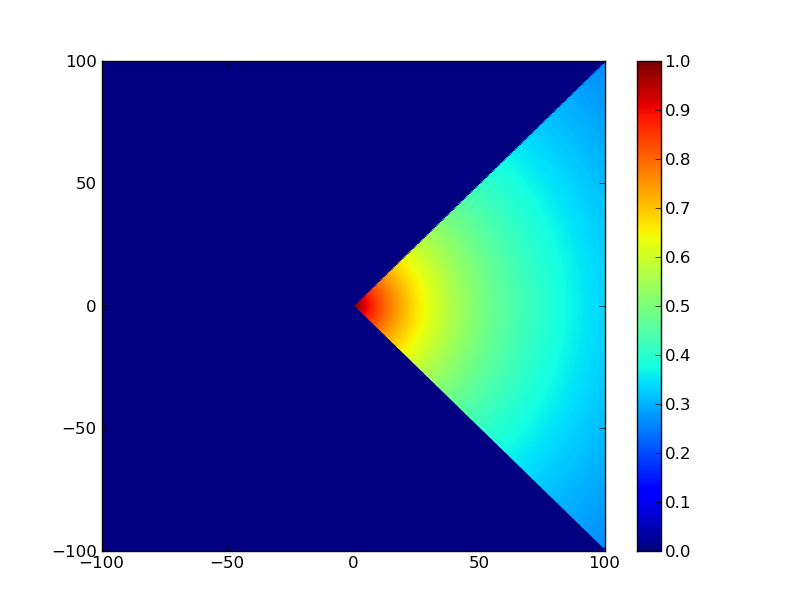
\includegraphics[width=0.48\textwidth]{graphs/proximity.png}
	\end{center}
	\vspace{-30pt}
	\caption{Proximity: $bias=50$ $\alpha=\pi/4$}
\end{wrapfigure}

\subsection{Smell}
\begin{wrapfigure}{r}{0.5\textwidth}
	\vspace{-30pt}
	\begin{center}
		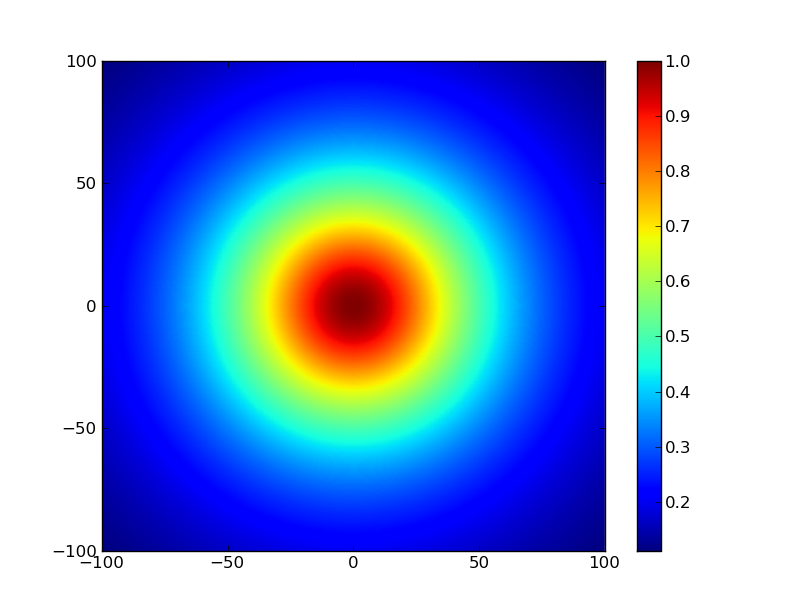
\includegraphics[width=0.48\textwidth]{graphs/smell.png}
	\end{center}
	\vspace{-30pt}
	\caption{Smell: $bias=50$}
\end{wrapfigure}

\subsection{Sound}
\begin{wrapfigure}{r}{0.5\textwidth}
	\vspace{-30pt}
	\begin{center}
		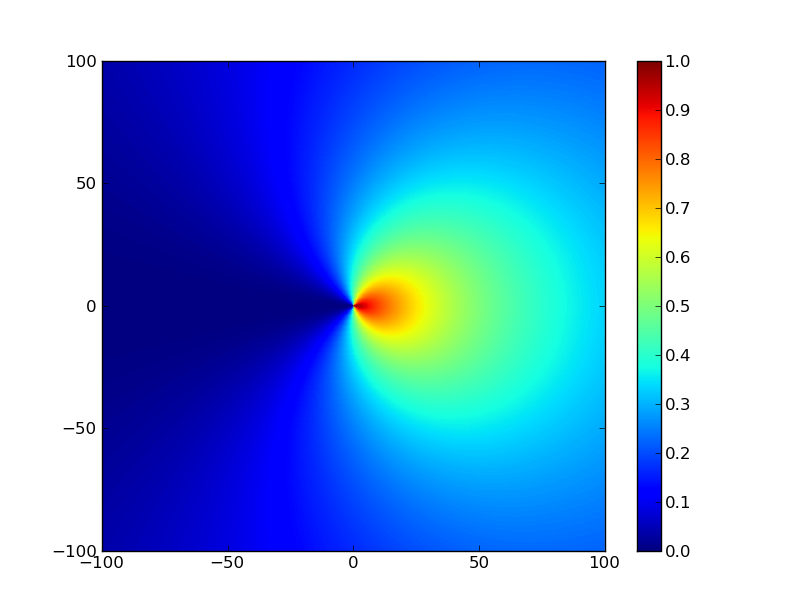
\includegraphics[width=0.48\textwidth]{graphs/cardioid.png}
	\end{center}
	\vspace{-30pt}
	\caption{Sound: $bias=50$}
\end{wrapfigure}

% TODO \subsection{Beam}

\cleardoublepage
\section{Vehicles}
\subsection{Eight}
\begin{wrapfigure}{r}{0.5\textwidth}
	\begin{center}
		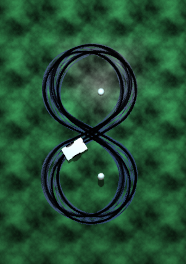
\includegraphics[width=0.48\textwidth]{trail/eight.png}
	\end{center}
	\caption{Trail of the eight vehicle}
\end{wrapfigure}

\subsection{Ellipse}
\begin{wrapfigure}{r}{0.5\textwidth}
	\begin{center}
		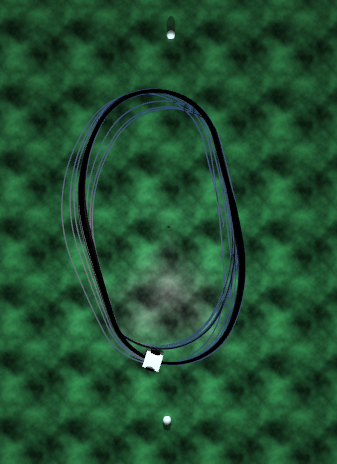
\includegraphics[width=0.48\textwidth]{trail/ellipse.png}
	\end{center}
	\caption{Trail of the ellipse vehicle}
\end{wrapfigure}

\subsection{Braitenberg 3c}

\cleardoublepage
\section{Project}


\end{document}
